\documentclass[12pt,a4paper]{article}
\usepackage[utf8]{inputenc}
\usepackage{amsmath}
\usepackage{amsfonts}
\usepackage{amssymb}

\usepackage{cmap} % для кодировки шрифтов в pdf
\usepackage[T1]{fontenc}
\usepackage{hhline}
\usepackage[unicode]{hyperref}
\usepackage{multirow}
\usepackage{array}
\usepackage{amsmath}
\usepackage{bm}
\usepackage{textcomp}
\usepackage[russian]{babel}
\usepackage{graphicx} % для вставки картинок
\usepackage{amssymb,amsfonts,amsmath,amsthm} % математические дополнения от АМС
\usepackage{indentfirst} % отделять первую строку раздела абзацным отступом тоже
% Поля
\usepackage{geometry}
\geometry{left=2cm}
\geometry{right=1.5cm}
\geometry{top=2.4cm}
\geometry{bottom=2.cm}

%%%%%%%%%%%%%%%%%%%%%%%%%%%%%%%     

\linespread{1.5} % полуторный интервал
\frenchspacing

\begin{document}
	
	\begin{titlepage}
		
		\begin{center}
			\begin{large}
				Санкт-Петербургский Политехнический университет\\ Петра Великого\\
				Институт прикладной математики и механики\\
			\end{large}
			\vspace{0.2cm}
			Высшая школа прикладной математики и вычислительной физики\\
			
		\end{center}
		
		\vspace{3cm}
		\begin{center}
			\textbf{Отчёт\\ по лабораторной работе 5\\ по дисциплине\\ "математическая статистика"}
		\end{center}
		
		\vspace{3cm}
		\vbox{%
			\hfill%
			\vbox{%0
				\hbox{Выполнил студент:}%
				\hbox{\break}
				\hbox{Аникин Александр Алексеевич,}%
				\hbox{группа 3630102$\backslash$80201}%
				\hbox{\break}
				\hbox{\break}
				\hbox{Проверил:}
				\hbox{\break}
				\hbox{к.ф.-м.н., доцент}
				\hbox{Баженов Александр Николаевич}
			}%
		} 
		\vfill
		
		\begin{center}
			Санкт-Петербург\\2021
		\end{center}
		
	\end{titlepage}
	\tableofcontents
	\newpage
	
	\listoffigures
	\newpage
	
	\listoftables
	\newpage	
	
	\section{Постановка задачи}
	Сгенерировать двумерные выборки размерами 20, 60, 100 для нормального двумерного распределения $N(x, y, 0, 0, 1, 1, \rho)$. Коэффициент корреляции взять равным 0, 0.5, 0.9. Каждая выборка генерируется 1000 раз и для неё вычисляются: среднее значение, среднее значение квадрата и дисперсия коэффициентов корреляции Пирсона, Спирмена и квадрантного коэффициента корреляции. Повторить все вычисления для смеси нормальных распределений:
	
	\begin{equation}\label{mixed_normal}
		f(x,y)=0.9N(x,y,0,0,1,1,0.9)+0.1N(x,y,0,0,10,10,-0.9).
	\end{equation} 
	Изобразить сгенерированные точки на плоскости и нарисовать эллипс рассеивания.
	\newpage
	
	\section{Теория}
		\subsection{Двумерное нормальное распределение}
			Двумерная случайная величина $(X, Y)$ называется распределённой нормально (или просто нормальной), если её плотность вероятности определена формулой

			\begin{equation}\label{bivariate_normal}
				N(x,y,\bar{x}, \bar{y}, \sigma_x, \sigma_y 	\rho)=\frac{\exp{(-\frac{1}{2(1-\rho^2)}[\frac{(x-\bar{x})^2}{\sigma_x^2}-2\rho\frac{(x-\bar{x})(y-\bar{y})}{\sigma_x\sigma_y} +\frac{(y-\bar{y})^2}{\sigma_y^2}])}}{2\pi \sigma_x \sigma_y \sqrt{1-\rho^2}}
			\end{equation}
			Компоненты $X, Y$ двумерной нормальной случайной величины также распределены нормально с математическими ожиданиями $\bar{x}, \bar{y}$ и средними квадратическими отклонениями $\sigma_x, \sigma_y$ соответственно (\cite{coeffs}, с. 133-134).
			Параметр $\rho$ называется коэффициентом корреляции:
			\begin{equation}
				\rho = \frac{K}{\sigma_x\sigma_y},
			\end{equation}
			где $K$ - корреляционный момент (иначе ковариация) случайных величин $X$ и $Y$:
			\begin{equation}
				K = cov(X, Y) = M[(X-\bar{x})(Y-\bar{y})]
			\end{equation}
		\subsection{Выборочные коэффициенты корреляции}
			\subsubsection{Коэффициент корреляции Пирсона}
				Выборочный коэффициент корреляции Пирсона:
				\begin{equation}\label{pearson}
					r_P = \frac{\sum_{i=0}^{n}(x_i-\bar{x})(y_i-\bar{y})}{\sqrt{\sum_{i=0}^{n}(x_i-\bar{x})^2\sum_{i=0}^{n}(y_i-\bar{y})^2}} = \frac{K}{S_X S_Y},
				\end{equation}
				где $S_X$ и $S_Y$ - дисперсии случайных величин $X$ и $Y$
			\subsubsection{Коэффициент корреляции Спирмена}
				Обозначим ранги, соответствующие значениям переменной $X$, через $u$, а ранги, соответствующие значениям переменной $Y$ , — через $v$.
				Выборочный коэффициент ранговой корреляции Спирмена:
				\begin{equation}\label{spearmen}
					r_S = \frac{\sum_{i=0}^{n}(u_i-\bar{u})(v_i-\bar{v})}{\sqrt{\sum_{i=0}^{n}(u_i-\bar{u})^2\sum_{i=0}^{n}(v_i-\bar{v})^2}},
				\end{equation}
				где $\bar{u} = \bar{v} = \frac{1 + 2+...+n}{n} = \frac{n+1}{2}$ - среднее значение рангов (\cite{coeffs}, с. 540-541).
			\subsubsection{Квадрантный коэффициент корреляции}		
				Выборочный квадрантный коэффициент корреляции:
				\begin{equation}\label{quadrant}
					r_Q = \frac{(n_1 + n_3)-(n_2+n_4)}{n},
				\end{equation}
				где $n1, n2, n3, n4$ — количества точек с координатами $(x_i, y_i)$, попавшими
				соответственно в $I, II, III, IV$ квадранты декартовой системы с осями $x'=x-med(x)$, $y'=y-med(y)$ и с центром в точке $(med(x), med(y))$ (\cite{coeffs}, с. 539).
		\subsection{Эллипс рассеивания}
			Уравнение проекции эллипса рассеивания на плоскость $xOy$:
			\begin{equation}\label{ellipse}
				\frac{(x-\bar{x}^2)}{\sigma_x}-2\rho\frac{(x-\bar{x})(y-\bar{y})}{\sigma_x\sigma_y} + \frac{(y-\bar{y})^2}{\sigma_y^2} = c, \qquad c=const
			\end{equation}
			Принцип выбора константы $c$:\\
			Выразим из уравнения $y$:\\
			\begin{equation}
				y_{1, 2} = \sigma_y\Bigg(\rho\frac{x-\bar{x}}{\sigma_x}\pm\sqrt{\frac{(x-\bar{x})^2}{\sigma_x^2}(\rho^2-1)+c}\Bigg)+\bar{y}
			\end{equation}
			Заметим, что 
			\begin{equation}
				\frac{(x-\bar{x})^2}{\sigma_x^2}(\rho^2-1)+c \geq 0
			\end{equation}
			поэтому
			\begin{equation}
				c = \max({-\frac{(x_i-\bar{x})^2}{\sigma_x^2}(\rho^2-1)}), \qquad i = 1, ... , n
			\end{equation}

	\newpage
	
	\section{Реализация}
		Лабораторная работа выполнена на языке Python 3.8 с помощью загружаемых пакетов SciPy, MatPlotLib, NumPy. Исходный код лабораторной работы находится на GitHub репозитории.
	\newpage
	
	\section{Результаты}
		\subsection{Выборочные коэффициенты корреляции}
		
			\begin{table}[htp]
			\label{coeffs_default_20}
				\begin{center}
					\begin{tabular}{|c|c|c|c|}
						\hline						
						$\rho$ = 0 & $r_P$[\ref{pearson}] & $r_S[\ref{spearmen}]$ & $r_Q$[\ref{quadrant}] \\ \hline
						$E(z)$ & 0.003 & 0.005 & 0.002 \\ \hline
						$E(z^2)$ & 0.053 & 0.055 & 0.050 \\ \hline
						$D(z)$ & 0.053 & 0.055 & 0.050 \\ \hline
						
						$\rho$ = 0.5 & $r_P$ & $r_S$ & $r_Q$ \\ \hline
						$E(z)$ & 0.485 & 0.457 & 0.319 \\ \hline
						$E(z^2)$ & 0.267 & 0.246 & 0.145 \\ \hline
						$D(z)$ & 0.031 & 0.0376 & 0.043 \\ \hline
						
						$\rho$ = 0.9 & $r_P$ & $r_S$ & $r_Q$ \\ \hline
						$E(z)$ & 0.895 & 0.865 & 0.717 \\ \hline
						$E(z^2)$ & 0.803 & 0.752 & 0.538 \\ \hline
						$D(z)$ & 0.002 & 0.005 & 0.025 \\ \hline
						
					\end{tabular}
				\end{center}
			\caption{Нормальное двумерное распределение [\ref{bivariate_normal}], 20 элементов}
			\end{table}
			\newpage
		
			\begin{table}[htp]
			\label{coeffs_default_60}
				\begin{center}
					\begin{tabular}{|c|c|c|c|}
						\hline	
						$\rho$ = 0 & $r_P$ & $r_S$ & $r_Q$ \\ \hline
						$E(z)$ & -0.002 & -0.001 & 0.001 \\ \hline
						$E(z^2)$ & 0.016 & 0.017 & 0.017 \\ \hline
						$D(z)$ & 0.016 & 0.017 & 0.017 \\ \hline
						
						$\rho$ = 0.5 & $r_P$ & $r_S$ & $r_Q$ \\ \hline
						$E(z)$ & 0.500 & 0.478 & 0.339 \\ \hline
						$E(z^2)$ & 0.259 & 0.239 & 0.129 \\ \hline
						$D(z)$ & 0.009 & 0.011 & 0.014 \\ \hline
						
						$\rho$ = 0.9 & $r_P$ & $r_S$ & $r_Q$ \\ \hline
						$E(z)$ & 0.900 & 0.884 & 0.713 \\ \hline
						$E(z^2)$ & 0.811 & 0.783 & 0.517 \\ \hline
						$D(z)$ & 0.001 & 0.001 & 0.008 \\ \hline
						
					\end{tabular}
				\end{center}
			\caption{Нормальное двумерное распределение, 60 элементов}
			\end{table}	
	 		\newpage		
		
			\begin{table}[htp]
			\label{coeffs_default_100}
				\begin{center}
					\begin{tabular}{|c|c|c|c|}
						\hline	
						$\rho$ = 0 & $r_P$ & $r_S$ & $r_Q$ \\ \hline
						$E(z)$ & 0.001 & -0.001 & -0.002 \\ \hline
						$E(z^2)$ & 0.010 & 0.010 & 0.009 \\ \hline
						$D(z)$ & 0.010 & 0.010 & 0.009 \\ \hline
						
						$\rho$ = 0.5 & $r_P$ & $r_S$ & $r_Q$ \\ \hline
						$E(z)$ & 0.500 & 0.481 & 0.336 \\ \hline
						$E(z^2)$ & 0.255 & 0.237 & 0.122 \\ \hline
						$D(z)$ & 0.006 & 0.006 & 0.009 \\ \hline
						
						$\rho$ = 0.9 & $r_P$ & $r_S$ & $r_Q$ \\ \hline
						$E(z)$ & 0.899 & 0.885 & 0.709 \\ \hline
						$E(z^2)$ & 0.808 & 0.785 & 0.508 \\ \hline
						$D(z)$ & 0.0002 & 0.001 & 0.005 \\ \hline
			
					\end{tabular}
				\end{center}
			\caption{Нормальное двумерное распределение, 100 элементов}
			\end{table}
			\newpage
		
			\begin{table}[htp]
				\label{coeffs_mixed_20}
				\begin{center}
					\begin{tabular}{|c|c|c|c|}
						\hline
						$n=20$ & $r_P$ & $r_S$ & $r_Q$ \\ \hline
						$E(z)$ & -0.099 & -0.091 & -0.056 \\ \hline
						$E(z^2)$ & 0.057 & 0.055 & 0.050 \\ \hline
						$D(z)$ & 0.048 & 0.047 & 0.047 \\ \hline
						
						$n=60$ & $r_P$ & $r_S$ & $r_Q$ \\ \hline
						$E(z)$ & -0.101 & -0.096 & -0.066 \\ \hline
						$E(z^2)$ & 0.027 & 0.026 & 0.021 \\ \hline
						$D(z)$ & 0.017 & 0.016 & 0.017 \\ \hline
						
						$n=100$& $r_P$ & $r_S$ & $r_Q$ \\ \hline
						$E(z)$ & -0.099 & -0.094 & -0.065 \\ \hline
						$E(z^2)$ & 0.019 & 0.019 & 0.014 \\ \hline
						$D(z)$ & 0.010 & 0.010 & 0.010 \\ \hline
					\end{tabular}
				\end{center}
			\caption{Смешанное нормальное двумерное распределение[\ref{mixed_normal}]}
			\end{table}
			\newpage
			
		\subsection{Эллипсы рассеивания}
			\centering{
				\begin{figure}[htp]
					\begin{minipage}[h]{0.25\linewidth}
						\centering{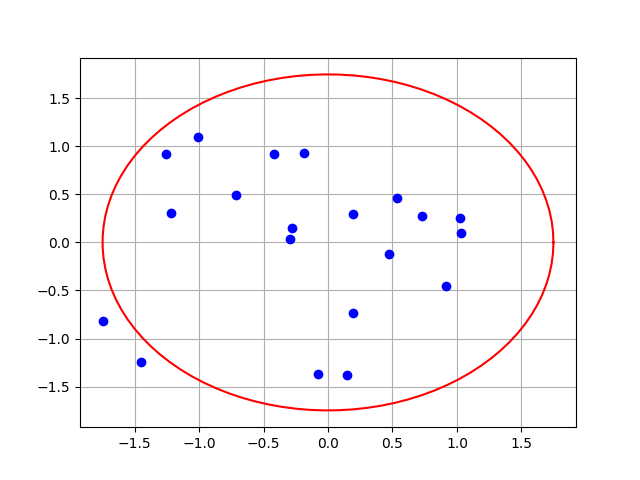
\includegraphics[width=1.25\linewidth]{./../plots/20_00.png}\\\centering{$\rho=0$}}
					\end{minipage}
					\hfill
					\begin{minipage}[h]{0.25\linewidth}
						\centering{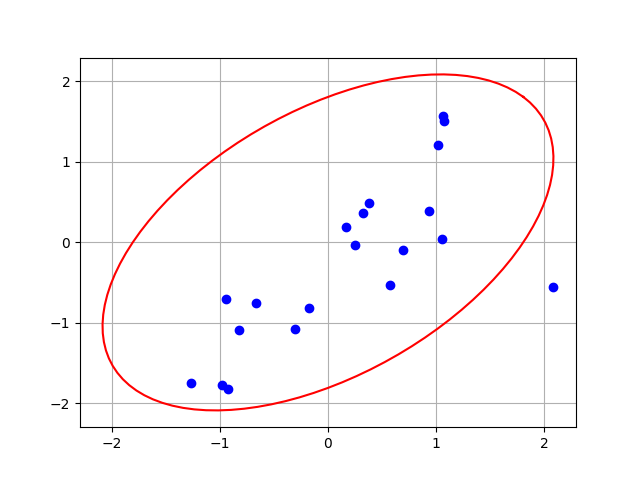
\includegraphics[width=1.25\linewidth]{./../plots/20_05.png}\\\centering{$\rho=0.5$}}
					\end{minipage}
					\hfill
					\begin{minipage}[h]{0.25\linewidth}
						\centering{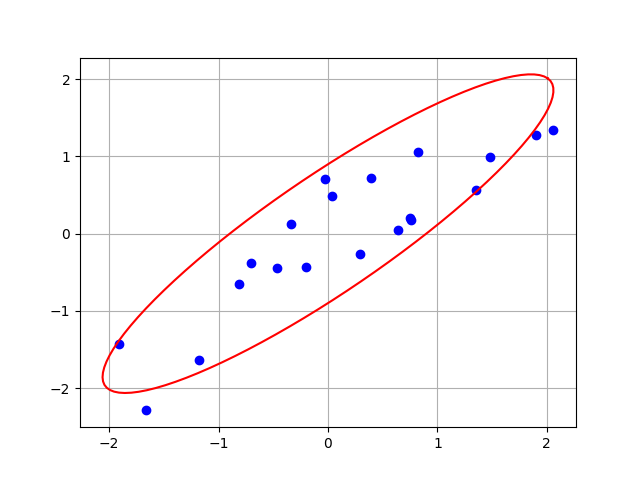
\includegraphics[width=1.25\linewidth]{./../plots/20_09.png}\\\centering{$\rho=0.9$}}
					\end{minipage}
					\caption{Эллипсы рассеивания [\ref{ellipse}] для выборки из 20 элементов}
					\label{ellipse_20}
				\end{figure}
			}
		
		\centering{
			\begin{figure}[htp]
				\begin{minipage}[h]{0.25\linewidth}
					\centering{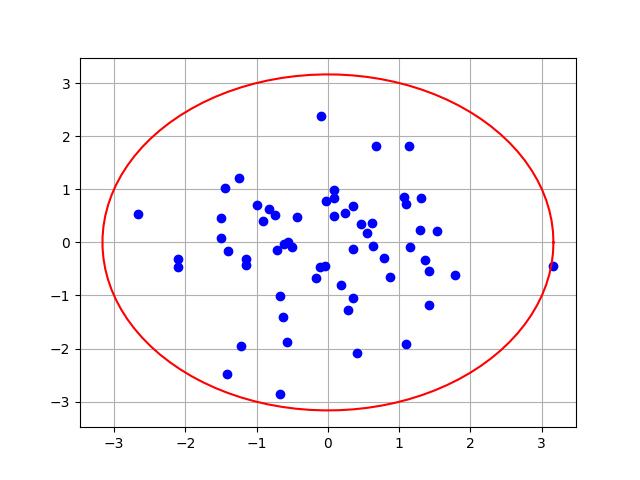
\includegraphics[width=1.25\linewidth]{./../plots/60_00.png}\\\centering{$\rho=0$}}
				\end{minipage}
				\hfill
				\begin{minipage}[h]{0.25\linewidth}
					\centering{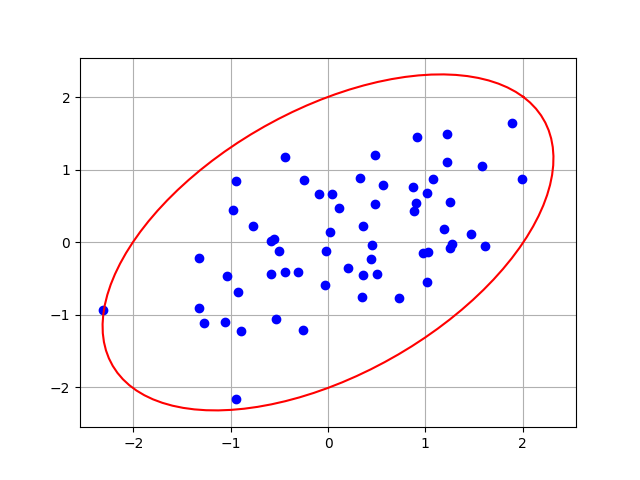
\includegraphics[width=1.25\linewidth]{./../plots/60_05.png}\\\centering{$\rho=0.5$}}
				\end{minipage}
				\hfill
				\begin{minipage}[h]{0.25\linewidth}
					\centering{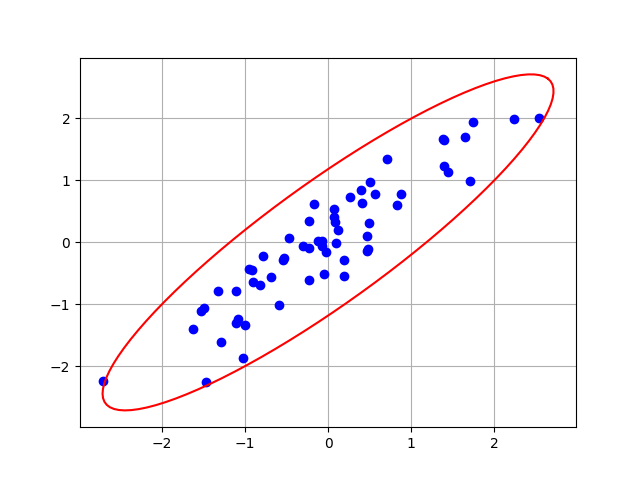
\includegraphics[width=1.25\linewidth]{./../plots/60_09.png}\\\centering{$\rho=0.9$}}
				\end{minipage}
				\caption{Эллипсы рассеивания для выборки из 60 элементов}
				\label{ellipse_60}
			\end{figure}
		}
		
		\centering{
			\begin{figure}[htp]
				\begin{minipage}[h]{0.25\linewidth}
					\centering{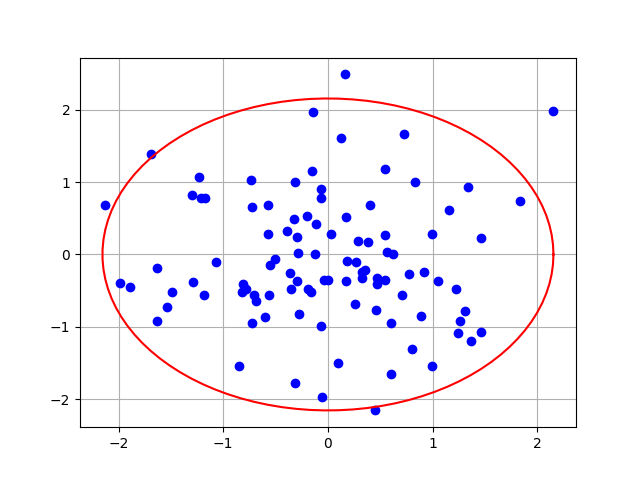
\includegraphics[width=1.25\linewidth]{./../plots/100_00.png}\\\centering{$\rho=0$}}
				\end{minipage}
				\hfill
				\begin{minipage}[h]{0.25\linewidth}
					\centering{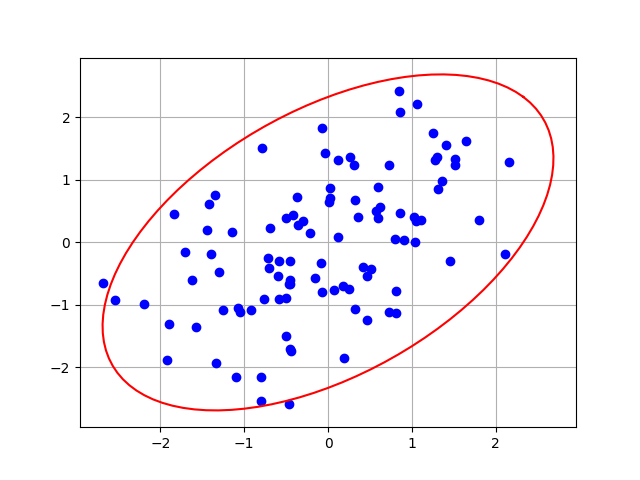
\includegraphics[width=1.25\linewidth]{./../plots/100_05.png}\\\centering{$\rho=0.5$}}
				\end{minipage}
				\hfill
				\begin{minipage}[h]{0.25\linewidth}
					\centering{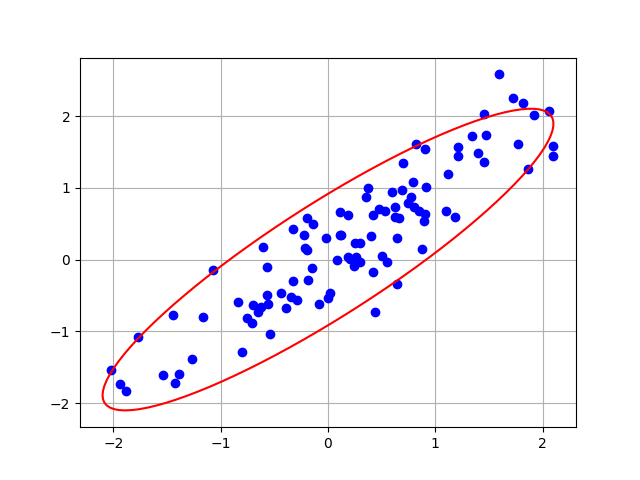
\includegraphics[width=1.25\linewidth]{./../plots/100_09.png}\\\centering{$\rho=0.9$}}
				\end{minipage}
				\caption{Эллипсы рассеивания для выборки из 100 элементов}
				\label{ellipse_100}
			\end{figure}
		}
	\clearpage
	\newpage
	
	\begin{flushleft}
		\begin{thebibliography}{1}
			\addcontentsline{toc}{section}{\bibname}
			\bibitem{coeffs}  Вероятностные разделы математики. Учебник для бакалавров технических направлений.//Под ред. Максимова Ю.Д. — Спб.: «Иван Федоров»,
			2001. — 592 c., илл.
		\end{thebibliography}
	\end{flushleft}
	
\end{document}